\chapter{Feature Based Design Model}


	\section{Introduction}

	Models are basically approximations of some real world situation, object or
	concept. A model consists of the information that is needed by the 
	application and all other parameters are ignored. The success of a CAD 
	model depends on the following factors :

	\begin{enumerate}
	\item
	Capturing designer's intent
	\item
	Simplicity
	\item
	Potential to create physically realizable objects 
	\item
	Rich set of operators to manipulate the created objects
	\item
	Robustness
	\end{enumerate}

	Most conventional solid modelers use a data structure that can model a 
	large variety of shapes. Though advantageous in the sense of 
	{\em completeness}, they are often lacking in terms of efficiency while 
	working with parts that have relatively simple geometry. 
	Efforts devoted to formalizing methods that operate on any generalized 
	shape tend to be complex and cumbersome for simpler shapes. 
	Thus, it may be possible to exploit the simplicity of a family of 
	components to great advantage. One of the most common and relatively 
	unexploited part families is the family of block-structured parts. 
	The present work further restricts this family to the class of
	generalized orthohedral block-structured parts.


	\section{Orthohedral block-structure}

	An orthohedral block-structured object is one which only contains faces
	that are perpendicular to a coordinate axis. Orthohedral geometry makes
	it easier to decompose a component into a set of rectangular blocks 
	positioned
	relative to each other. As the planes of attachment are finite and
	simple (each being perpendicular to a coordinated axis), positioning takes 
	less effort than positioning more complex shapes.


	It is clear that pure orthohedral geometry is not sufficient for
	modeling mechanical parts, since curved and sloping surfaces are often 
	necessary. To take advantage of a {\em simplicity} offered by the 
	orthohedral
	block-structure and still have the capability to model shapes with curved
	and sloping surfaces, a combined data representation is proposed. In this
	data representation, the shape of the part is decomposed into two aspects :

		\begin{enumerate}
		\item
		External shape
		\item
		Internal shape
		\end{enumerate}

	The external shape has the orthohedral block-structure, while the internal
	shape defines the actual geometry of the part. A mapping is defined 
	between the external shape and the internal shape. Additional parameters 
	may be
	needed to define the internal geometry with respect to the external block.
	Once the external shape gets defined completely, the mapping takes care of 
	the
	internal details and thus {\em encapsulates} the inner geometry. This
	idea of {\em encapsulation} is dealt with in more detail later in this
	thesis.

	Orthohedral block-structured geometry offers the following advantages :

		\begin{itemize}
		\item
		{\em Creation} : Easier to position blocks with respect to each other.
		\item
		{\em Editing} : Locational editing is simple to perform. Mapping 
						between
						external and internal shape takes care of transmitting 
						editing changes to internal geometry.
		\item
		{\em Display} :	Time is saved by displaying block-wise in the initial
						stages of modeling.
		\item
		{\em Object-oriented implementation} : Extension of shapes is easier
						as only a new {\em mapping} needs to be defined. The
						new shape can still use all the old functions that
						were applicable to the external shape.
		\end{itemize}


	\section{Data Representation}
		
	The data representation scheme that is proposed here is an extension of the
	approach followed by Hijazi~\cite{Hijazi}, Chennapragada~\cite{Venky},
	and Yang~\cite{Yang}. In this scheme, a component is considered to be a 
	set of blocks interconnected by topological links and is perceived as a 
	solid. In the following sections, the basic data structure is explained in 
	more detail.


	Any representation scheme for generalized orthohedral components must
	handle two principal types of data related to the shape of the component :
	geometric data and topological data. Geometric data defines the shape and 
	size parameters while topological data defines the size independent 
	connectivity 
	relationships among primitive features.

	
	In our model, the geometric data is contained in the blocks that make up a
	component and the topological data is contained in the topological links.

        \begin{figure}[htbp]
            %\centerline{\psfig{figure=datarep.ps,width=4.0in,height=6.0in}}
            \includegraphics{DATAREP.pdf}
            \caption{Data Representation}
            \label{datarep}
        \end{figure}

	Figure ~\ref{datarep} shows the decomposition of data information into
	geometric and topological information. The geometry contains plane values
	with respect to a global coordinate system, while topology contains the type
	of connectivity between the blocks.

	
	The representation of blocks and topological links is detailed in the
	following sections.

	\subsection{Blocks} 

	The geometry of a block is divided into two parts, viz., external geometry
	and internal geometry. External geometry is represented by a rectangular
	parallelopiped block which adheres to the idea of orthohedral 
	block-structured geometry. All topological connectivities are defined
	with respect to the external shape and are thus independent of the 
	internal geometry of the block. Internal geometry represents the actual
	shape of the block, which may or may not be the same as the external shape.
	Functionality like display, local edit, and volume computation are specific
	to the internal shape. For example, a cylinder can be decomposed into
	an external shape and an internal shape as shown in Figure ~\ref{cylblk}.

        \begin{figure}[htbp]
        	\hspace{2.5cm}
	% \centerline{\psfig{figure=cylblk.ps,width=3.0in,height=3.0in}}
	\includegraphics[width=3.0in,height=3.0in]{CYLBLK.pdf}
            \caption{External and Internal Shape}
            \label{cylblk}
        \end{figure}

	\subsubsection{Basic External Shape }

		Each object is assumed to be encapsulated in a rectangular block defined
	by a set of nine planes and three lengths. Orthohedral geometry means that 
	each plane is perpendicular to one of the three coordinate axes of the 
	global Cartesian coordinate system (Fig. ~\ref{Iyad16}). 
	Each axis is intersected by three planes denoted as MIN (minimum), 
	MID (middle) and MAX (maximum). The length of the block along a 
	particular axis, denoted Length, is defined as the distance between the MIN 	and the MAX planes along that axis. Three MAX planes (Xmax, Ymax, Zmax) 
	along with three MIN planes (Xmin, Ymin, Zmin) define the bounding planes 
	of the basic external shape.



		\begin{figure}[htbp]
%  			\centerline{\psfig{figure=iyad16.ps,width=4.0in,height=4.0in}}
 			\includegraphics{IYAD16.pdf}
  			\caption{A representation of the MIN, MID, and MAX planes.}
  			\label{Iyad16}
		\end{figure}


	The MID planes (Xmid, Ymid, Zmid) and the Lengths (Xlen, Ylen, Zlen) are 
	implicitly defined with respect to the MAX and the MIN planes. 
	The MID planes and the Length are redundant parameters which are maintained 
	because
	it may sometimes be easier to define the
	block using one or both of these parameters. Some topological
	links use the MID planes for link specification. The MID planes 
	explicitly define the position of a block with respect to the global 
	coordinate system.
	The Length of the block helps in providing further explicit geometric
	information about the size. Given any two parameters along an axis, the 
	other two can be 
	computed. This is done to reduce the input required and insure that
	geometric consistency is maintained. 

	The external shape is used to define topological relationships and 
	the relative position between two blocks. For all blocks, the user has to 
	define the external shape completely first and then specify the parameters 
	related to the internal shape. For a rectangular block, the external shape 
	itself acts as the internal shape and no further information is necessary 	
	to complete the definition.

    \subsubsection{Internal Shapes}

    The internal shape specifies the geometry of the feature with respect to
    the external shape. This is done by providing a mapping between the external
	rectangular shape and the internal geometry. Some additional data 
	may be necessary to complete the geometry definition. This gives us a
	way to extend the shape library and develop customized shapes. The internal
	shape is encapsulated within the external shape and thus remains local to 
	the block.


	The internal shape does not take part in global positioning of the
	block and does not participate in any topological links. 
	They contribute only to the operations that are {\em shape specific},
	such as display and volume calculations.


	Once the external shape gets defined, the additional input needed depends 
	on the type of the block. The prototype system developed by Hijazi
	~\cite{Hijazi}
    had only a constructive block feature. Later Chennapragada~\cite{Venky}
    extended the feature library to include subtractive blocks and cylinders. 
    The present work develops a hierarchy of shapes having blocks, cylinders, 
	wedges and extruded B-Spline surfaces.

	\subsection{Constructive and Subtractive Features}

	Constructive features can be defined as features in which the normals
	to the faces are outward from the block. Constructive features represent
	{\em solid} volume and constitute the primary structural building blocks.

	Subtractive features can be defined as features in which the normals
	to the faces are directed inward towards the block. Subtractive features
	represent voids. In the current prototype system,
	the subtractive features are implemented as derived classes of their
	corresponding constructive feature classes. The different {\em normal}
	directions for constructive feature faces and subtractive feature
	faces are achieved by linking vertices in the counterclockwise direction in
	case of the constructive features and in the clockwise direction in the 
	case of the subtractive features.

	Subtractive features differ from constructive features in the way the
	resting plane is assigned to the new feature from the existing feature.
	The assignment of the planes in the case where both the new and the
	existing features are subtractive is similar to the case where both are
	constructive features.


        \begin{figure}[htbp]
%            \centerline{\psfig{figure=addsub.ps,width=2.0in,height=6.0in}}
	\hspace{2.5cm}	
	\includegraphics{ADDSUB.pdf}
            \caption{Constructive and Subtractive feature plane assignment}
            \label{addsub}
        \end{figure}

	Figure ~\ref{addsub} shows the difference in plane assignment in the case of
	a {\em center face match} topological link. In case A, the MAX plane of 
	block-1
	matches with the MIN of block-2, while in case B, the MAX of block-1
	matches with the MAX of block-2. Similar differences occur for
	other topological links.	

	The current implementation provides subtractive block, subtractive cylinder
	and subtractive wedge features.


	\subsection{Topological Links }

	Topology defines relationships that must exist regardless of size between 
	the external shapes
	of different blocks in the component. In the current implementation, six 
	types of topological relations are developed, all of which are symmetrical
	in nature, i.e.
		\begin{quote}
		if $\sim$ is a topological relation, then \\
		A $\sim$ B $\Longleftrightarrow$ B $\sim$ A \\
		where A and B are the blocks involved in the relationship.

		\end{quote}

        \begin{figure}[htbp]
%            \centerline{\psfig{figure=symm.ps,width=2.0in,height=3.0in}}
	\hspace{2.5cm}
	\includegraphics[width=2.0in,height=3.0in]{SYMM.pdf}
            \caption{Symmetric Nature of the topological links}
            \label{symm}
        \end{figure}

        For example, if a block A
        is two corner matched with a block B, then block B is also two corner
        matched with block A. Figure ~\ref{symm} shows an example of a two 
		corner
        match with its graph representation. The graph reflects the symmetric
        nature of the topological links. A complete description of all the
		topological links that are supported is given below. The plane
		assignments in all cases are for a link between two constructive blocks.

	\begin{enumerate}

	\item
	Center Face Match [CFM] (Figure ~\ref{cfm})

        \begin{figure}[htbp]
%            \centerline{\psfig{figure=cfm.ps,width=2.0in,height=2.0in}}
	\hspace{4cm}
	\includegraphics{CFM.pdf}
	\caption{Center Face Match}
            \label{cfm}
        \end{figure}
 
		A MAX plane of one block is aligned with the MIN plane of the second 
		block along the same axis. In addition, the two MID planes of the 
		first block which are perpendicular to the other two axes are aligned 
		with the corresponding planes in the second block.

	\item
	Center Edge Match [CEM] (Figure ~\ref{cem})

        \begin{figure}[htbp]
%            \centerline{\psfig{figure=cem.ps,width=2.0in,height=2.0in}}
	\hspace{4cm}
	\includegraphics{CEM.pdf}
	\caption{Center Edge Match}
            \label{cem}
        \end{figure}
 
		The MAX plane of one block is aligned with the MIN plane of the second 
		block that is perpendicular to the same axis. In addition, a MAX
		of the first block is aligned with the MAX plane of the second block
		or a MIN plane of the first block is aligned with the MIN plane of the
		second block which is perpendicular to a second axis. The MID planes
		along the third axis are also aligned.

	\item
	One Corner Match [OCM]	(Figure ~\ref{ocm})

        \begin{figure}[htbp]
%            \centerline{\psfig{figure=ocm.ps,width=2.0in,height=2.0in}}
	\hspace{4cm}
	\includegraphics{OCM.pdf}
	\caption{One Corner Match}
            \label{ocm}
        \end{figure}
 
		The MAX plane of one block is aligned with the MIN plane of the second 
        block that is perpendicular to the same axis. In addition, a MAX plane
		and one of the MIN planes of the first block which are perpendicular to
		the other two coordinate axes, are aligned with the corresponding planes
		in the second block.

	\item
	Two Corner Match [TCM]	(Figure ~\ref{tcm})

        \begin{figure}[htbp]
%            \centerline{\psfig{figure=tcm.ps,width=2.0in,height=2.5in}}
	\hspace{4cm}
	\includegraphics{TCM.pdf}
	\caption{Two Corner Match}
            \label{tcm}
        \end{figure}
 
		The MAX plane of one block is aligned with the MIN plane of the second 
        block that is perpendicular to the same axis. In addition, either
		two MAX planes and one of the MIN planes of the first block are
		aligned with the corresponding planes of the second block or
		two MIN planes and one of the MAX planes of the first block are
		aligned with the corresponding planes of the second block.
 
	\item
	Four Corner Match [FCM]	(Figure ~\ref{fcm})

        \begin{figure}[htbp]
%            \centerline{\psfig{figure=fcm.ps,width=2.0in,height=2.0in}}
	\hspace{4cm}
	\includegraphics{FCM.pdf}
	\caption{Four Corner Match}
            \label{fcm}
        \end{figure}
 
		The MAX plane of one block is aligned with the MIN plane of the second 
        block that is perpendicular to the same axis. In addition, two MAX
		planes and two MIN planes perpendicular to the other two coordinate 
		axes are aligned with the corresponding planes in the second block.

	\item
	Shared Plane Match [SPM] (Figure ~\ref{spm})

        \begin{figure}[htbp]
%            \centerline{\psfig{figure=spm.ps,width=2.0in,height=2.0in}}
	\hspace{4cm}
	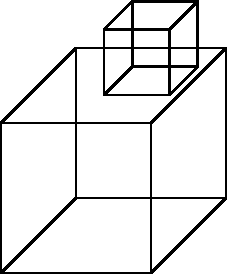
\includegraphics{SPM.pdf}
	\caption{Shared Plane Match}
            \label{spm}
        \end{figure}
 
		The MAX plane of one block is aligned with the MIN plane of the second 
        block that is perpendicular to the same axis.


	\end{enumerate}

	\subsubsection{Graph representation of the topology}

		Although a component can be conceptually represented as a collection of 
		blocks and a collection of topological links, this type of the model
		does not provide an adequate formal representation of the relationships 
		between the blocks and the topological links. Therefore, in our model,
		a component is represented as a list of blocks and a connected graph. 
		The graph is a directed graph, in which nodes represent blocks,
		and the incident edges represent the a topological links.
		The edges store information related to the topological link such as
		axis and type along with the information related to the type of 
		topological link. This is illustrated in Fig. ~\ref{compexa}.

        \begin{figure}[htbp]
%            \centerline{\psfig{figure=compexa.ps,width=5.0in,height=4.0in}}
	\includegraphics[scale=0.6]{compexa.png}
            \caption{Component and its graph representation}
            \label{compexa}
        \end{figure}




	\section{Operations}

	This section details some of the basic operations that must be supported
	in order to make the FBD system usable. All operations are discussed with
	respect to the data representation scheme that was presented in the 
	previous section.

	\subsection{Creation}

		The creation process can be broken down into three types :
		\begin{enumerate}
		\item
		Creation of a component
		\item
		Creation of a block
		\item
		Creation of a topological link
		\end{enumerate}

		\subsubsection{Creation of Components}
		
		The creation of a component is initiated by the creation of the first
		block purely from geometric data. This block will serve as the base to
		which other blocks can be added to form the desired component. 
		A list of blocks is maintained in the order in which they are added to 
		the 
		component. Most subsequent operations on the whole component traverse 
		the list of the blocks and perform the corresponding 
		operation at the block level. For example, displaying the component is 
		done by traversing the list of the blocks and displaying them in 
		order.

		\subsubsection{Creation of blocks}

		For purely geometric data input (as in the case of the initial block in
		a component) the user needs to specify two data values along each axis.
		The other two parameters are calculated internally. To add a block to 
		an existing component, the type of topology that will exist between the 		new block and at least one pre-existing block must be specified. 
		The establishment of this 
		topological link will result in the alignment of certain planes from
		the pre-existing block with the corresponding planes from the new block.
		Since the values of the planes involved in the topological link from the
		pre-existing block are known, the values of the corresponding planes
		in the new block are established. Therefore, a portion of the new 
		block's geometric data is defined, and the remaining data necessary to 
		complete the definition of this block must be provided. 
		This is done by prompting the user for the additional geometric data
		that is required.  Other blocks are added
		to the component in a similar manner until the desired component is
		generated. As each block is created, it is added to the list of blocks
		that make up the component.

		Many of the mechanical parts constituting an assembly bear geometric
		proportions with themselves or within other parts in the assembly. When
		there arises a need to modify any part dimensions, the related
		(linked) dimensions need to be changed to maintain the validity of the
		assembly. This automatic change in the dimensions of the parts that are
		geometrically related to the edited dimension can be achieved if there
		exist geometric length links between them. This 
		can be done in creation mode when the user is entering the length value
		of a feature, at which time he/she could be given the option of 
		linking this value to an existing one.
		This capability has not been implemented in the present work.

		\subsubsection{Creation of Topological links}

		Topological links specify the relative position of one block with
		respect to another.
		There are two ways in which topological links can be created :
		\begin{enumerate}
		\item
		Linking a new block to a pre-existing block
		\item
		Linking two pre-existing blocks
		\end{enumerate}
		Every topological link needs a base surface on which
		the contacting planes of the two blocks meet. Depending on the type of
		the topological link, more information may be requested to complete the
		definition of that link. The user may specify more than one topological
 		link between two blocks, provided they are compatible.
		Every topological link fixes the data of the second block with respect 
		to the first (base) block. In linking two pre-existing blocks, care 
		should be taken to ensure that their planes lie in such a way that 
		the requested
		topological link can be set up without changing the existing geometry.

	\subsection{Editing}

    There are two types of editing that are supported in this implementation :
    geometrical editing and topological editing. Geometrical editing involves 
	changing the shape parameters of the blocks and topological editing 
	involves changing the topological relations between the blocks.

	\subsubsection{Geometrical Editing} 

	Geometrical editing is performed at two levels.

        \begin{enumerate}
        \item
        External, which involves changes in the external shape of the block 
        \item
        Internal, which involves changes in the internal shape of the block
        \end{enumerate}


	The editing process can be broken down into the following major tasks :
	\begin{itemize}
		\item
		Selecting an object to modify
		\item
		Accepting a parameter to modify in the selected entity
		\item
		Validating the specified parameter 
		\item
		Actually performing the specified change in the parameter
		\item
		Propagating the change correctly through the component
	\end{itemize}

        \begin{figure}[htbp]
%            \centerline{\psfig{figure=editfcm.ps,width=3.0in,height=2.0in}}
	\hspace{4cm}
	\includegraphics[scale=0.8]{EDITFCM.pdf}
            \caption{Editing a component with Four Corner Match}
            \label{editfcm}
        \end{figure}

	For example, consider the component in Fig. ~\ref{editfcm}. 
	The following is the step by step
	process to change {\em Ylen} of Block 1, while keeping the Ymin plane of 
	Block 1 fixed.
	
	\begin{itemize}
		\item
		Select an object to modify :
						\begin{itemize}
						\item
						Block-Id = 1
						\item
						Axis = Y
						\item
						Parameter = Length
						\end{itemize}
		\item
		Present the value of old length and ask for new value, new-length.
		\item
		Validation of the input :
						\begin{itemize}
						\item
						If the new value is same as old value; no changes
						are performed.
						\item
						The new value should be a non-negative value.
						\end{itemize}
		\item
		Change the {\em Ylen} field to {\em new-length}.

		\item
		Propagation : As Block 2 is connected to Block 1 by the topo-link of 
		type
		{\em four corner match} along Y axis, modifying Ylen of Block 1 
		shifts the Ymax of Block 1 upwards. To maintain alignment,
		the Ymin and Ymax of Block 2 are shifted upwards by the same
		amount, new-length.

	\end{itemize}


    The graph structure used to model the component proves to be especially 
	advantageous in the editing  operations. The entire logic for editing
	can now be written as a well-structured graph algorithm~\cite{Howard}.


    Geometric editing involves much more than just changing the dimensions of
    the block selected by the user. Since the blocks are linked
    to each other by topological links, the changes in the dimensions of one 
	block may
    require changes in the dimensions of other blocks that are connected to it
	either directly or indirectly, in order to preserve the topology.

	
	\subsubsection{Difficulties in the Editing process}

	The editing process needs to be understood clearly so as to avoid ambiguity
	and un-wanted results. 
	Some of the issues that must be handled during the editing process are the
	following :

	\begin{itemize}
	\item
	Violation of topological links :


	During the editing of the component, if the geometry of a block is changed,
	some of the topological links may be violated unless other changes are made
	simultaneously. For example in Figure ~\ref{edittcma}, a topological link
	of the type Two Corner Match (TCM) exists between blocks 1 and 2. After
	performing a geometric change on the Xlength of block 1 while holding
	the Xmin plane fixed, this topological link will be violated as shown in
	Figure ~\ref{edittcmb}. Therefore all the blocks in the component must
	be visited to determine which of the topological links are violated,
	reestablish them, and perform appropriate geometric changes.
	
        \begin{figure}[htbp]
%            \centerline{\psfig{figure=iyad26a.ps,width=3.0in,height=3.0in}}
	\hspace{4cm}
	\includegraphics[width=3.0in,height=3.0in]{IYAD26A.pdf}
	\caption{Blocks with TCM before Editing }
            \label{edittcma}
        \end{figure}
 
        \begin{figure}[htbp]
%            \centerline{\psfig{figure=iyad26b.ps,width=3.5in,height=3.0in}}
	\hspace{4cm}
	\includegraphics[width=3.5in,height=3.0in]{IYAD26B.pdf}
            \caption{Blocks with TCM after Editing }
            \label{edittcmb}
        \end{figure}
 
	\item
	Specification of invariant plane :


	It is not sufficient to specify only the length to be changed; a plane
	of the block that remains invariant during the edit must be specified.
	For example, if Xlen (see Fig.~\ref{editpln}) of Block 1 is to
	be changed, the user has option of fixing one of the following planes.
		\begin{itemize}
		\item Xmin
		\item Xmid
		\item Xmax
		\end{itemize}
   
        \begin{figure}[htbp]
%            \centerline{\psfig{figure=editpln.ps,width=4.0in,height=5.0in}}
	\hspace{1cm}
	\includegraphics[width=4.0in,height=5.0in]{EDITPLN.pdf}
            \caption{Plane fixing in Editing}
            \label{editpln}
        \end{figure}

	\item
	Length Linking :

	If the length to be edited is linked to another length then the editing
	changes must occur in the second length to maintain the length relation. 
	Every length that is changed must be propagated to topologically linked 
	blocks; this should be correctly propagated during the editing process.
	Consider the example shown in Fig. ~\ref{lenlink}, with Length 1
	linked to Length 2. Suppose Length 1 is to be changed.
   
        \begin{figure}[htbp]
            %\centerline{\psfig{figure=lenlink.ps,width=2.0in,height=5.5in}}
	\hspace{4cm}
	\includegraphics[width=2.0in,height=5.5in]{LENLINK.pdf}
            \caption{Length Linking in Editing}
            \label{lenlink}
        \end{figure}


	The changes that occur when ``Length1'' is modified keeping Xmin fixed,
	are as follows
		\begin{itemize}
		\item
		To maintain the topological link of type ``Two Corner Match'' between
		block-1 and block-4, block-4 translates to the right.
		\item
		Because of length linking between ``Length-1'' and ``Length-2'', Ylen
		of block-4 gets modified keeping Ymin constant (say). So block-4
		extends in the upward direction. 
		\item
		To maintain the topological link of type ``Two Corner Match'' between
        block-3 and block-4, the block-3 translates upwards.
		\item
        To maintain the topological link of type ``Two Corner Match'' between
        block-3 and block-2, block-2 extends upwards.
		\end{itemize}

	The final configuration is shown in Fig. ~\ref{lenlink}(b).

	\item
	Cycles in a component :


	The previous example was a simple one in which the blocks in the 
	component are linked in a cycle. This can be seen in the graph of the 
	component shown in Figure ~\ref{cylegra}. The editing algorithm must be
	capable of handling components with any number of cycles and propagating
	the geometric changes correctly.

        \begin{figure}[htbp]
%            \centerline{\psfig{figure=iyad28.ps,width=3.0in,height=5.0in}}
	\hspace{4cm}
	\includegraphics{IYAD28.pdf}
            \caption{Cycle in Graph}
            \label{cylegra}
        \end{figure}
 

	For example, a Two Corner Match exists between blocks 1 and block 4 in 
	Figure
	~\ref{cylegra}. Suppose the user wants to edit the Xlength of block 1 
	with the Xmid plane fixed (Figure ~\ref{cyledita}). As Xlength increases 
	with Xmid fixed, Xmin of block 1 shifts to the left and Xmax of block-1 
	shifts to the right. To maintain the Two Corner Match between block-1 and 
	block-2, Xmin and Xmax of block-2
	move to the left, keeping its Xlength fixed. Similarly, to maintain the 
	Two Corner Match between block-1 and block-4, Xmin and Xmax of block-4 
	shift to 
	the right. It is clear from Figure ~\ref{cyleditb} that
	to maintain the topological consistency between block-2
	block-3 and between block-4 \& block-3, a change in the Xlength of 
	block-3 (Figure ~\ref{cyleditb}) is necessary. After the selection of 
	block-3
	as the modification node, the new length is internally calculated to
	satisfy both the topological links. During this process it is assumed that :

		\begin{itemize}
		\item
		Only one length is allowed to be changed per cycle
		\item
		The user selects a correct node for the modification of length.
		\item
		If the edit is possible without modifying any length, it
		will be done in this way.
		\end{itemize}

        \begin{figure}[htbp]
%            \centerline{\psfig{figure=cyledita.ps,width=3.0in,height=3.0in}}
	\hspace{4cm}
	\includegraphics[width=3.0in,height=3.0in]{CYLEDITA.pdf}
            \caption{Component having Cycle before editing}
            \label{cyledita}
        \end{figure}
 
        \begin{figure}[htbp]
%            \centerline{\psfig{figure=cyleditb.ps,width=3.0in,height=3.0in}}
	\hspace{4cm}
	\includegraphics[width=3.0in,height=3.0in]{CYLEDITB.pdf}
            \caption{Inconsistency in Component editing having Cycle}
            \label{cyleditb}
        \end{figure}
 

	\end{itemize}

	\subsection{Algorithm for Editing}

	Before presenting the method of traversal used in the editing process,
	several variables must be first defined.

	\begin{itemize}
	\item
	{\em Fixed} : A boolean variable associated with the lengths and planes of
	a block. This variable is set to ``true'' when the blocks are initially
	created. If this variable is ``false'', the value of the length or the plane
	can be changed.
	\item
	{\em Resolved} : A boolean variable associated with each graph node. This
	variable is set to ``true'' when all the planes and lengths constituting
	the block that the node represents have their {\em Fixed} variable
	set to ``true''.
	\item
	{\em Visited} : A boolean variable associated with each node. This variable
	is set to ``true'' when all cycles that the node is a member of have been
	traversed, and all adjacent nodes have their {\em Resolved} variable
	set to ``true''.
	\item
	{\em Modify} : A boolean variable associated with each node. This variable
	is set to ``true'' if the node is part of a cycle and its length is
	allowed to be modified.
	\item
	{\em Base node} : A node is labeled as the {\em Base node} when it is
	the current node removed from the queue of the nodes to be visited during
	the editing process.
	\item
	{\em Update} : A procedure that recalculates the values of those lengths
	and planes of a block that have their {\em Fixed} field set to ``false''.
	After recalculating their values, {\em Update} sets their {\em Fixed}
	variable to ``true''.
	\end{itemize}

	Before each graph traversal, the graph is decomposed into strong-components
	to find all possible fundamental cycles ~\cite{Rein}, and sets all the
	boolean variables to ``false''. The steps of the algorithm are as
	follows :

	\begin{enumerate}

	\item
	The block and length are selected for modification. The user inputs
	new length value denoted as {\em new-length} and {\em axis} along which
	length is to be modified. The node representing
	the edited block is labeled as the {\em edited node}.

	\item
	Three queues are set up corresponding to the three coordinated axes, viz.,
	XQ, YQ, and ZQ.
	Function Change-Length({\em edited node, axis, new-length} )( see Sec.
	~\ref{chglen}) is called which returns B.

	\item
	If B = ``true'',
		\begin{itemize}
		\item
		The {\em edited node} is put in the corresponding {\em axis} queue, 
		which is then set as the current queue.
		\end{itemize}
	Else,
		\begin{itemize}
		\item
		Exit.
		\end{itemize}
	\item
	\label{edthr}
	If all queues are empty,
		\begin{itemize}
		\item
		Exit.
		\end{itemize}
	If the {\em current queue} is empty, 
		\begin{itemize}
		\item
	The other queues are searched.
		\item
	The first non-empty queue is made the {\em current queue}.
		\end{itemize}

	\item
	The head of the {\em current queue} is removed from the queue and set as
	the current {\em Base node}.

	\item
	\label{start}
	If the {\em Base node's Visited} variable is ``false'', 
		\begin{itemize}
		\item
		Non-redundant cycles of length more than two which contain the 
		{\em Base node} are found and listed.
		\end{itemize}
	Else,
		\begin{itemize}
		\item
		Go to step ~\ref{edthr}.
		\end{itemize}

	\item
	The user is allowed to specify the order in which the listed cycles are
	to be processed.

	\item
	For the selected cycle, the user is prompted to select a suitable 
	{\em modification
	node}. The {\em Modify} variable of that node is set to ``true'' (
	If the selected node has its {\em Resolved} variable or {\em Visited}
	variable set to ``true'', an error message is given and the user is asked
	to select another {\em modification node}).

	\item
	\label{edeight}
	Set the cycle traversal direction to be ``forward'' (i.e.
	the direction in which the nodes in the cycle are listed). The node next
	to the {\em Base node} is made the {\em current node}.

	\item
	\label{ednine}
	If the {\em current node} is the {\em Base node}, 
		\begin{itemize}
		\item
		Go to step ~\ref{edfort}.
		\end{itemize}
	Else, if the {\em current node} is the {\em modification node} and
		if one of the planes in the direction of {\em axis} have {\em Fixed}
		variable value as ``true'',
		\begin{itemize}
		\item
		Go to step ~\ref{edtw}.
		\end{itemize}
		else,
		\begin{itemize}
		\item
		Partially resolve the {\em current node} by setting {\em Fixed} variable
		of the appropriate plane (based on available topological link 
		information) to ``true'' in the direction of the {\em axis}.
		\item
		Go to step ~\ref{edelv}.
		\end{itemize}
	Else,
		If the {\em current node} has its {\em resolved} variable set to 
		``true'', 
		\begin{itemize}
			\item
			An error message is given,
			\item
			Exit.
		\end{itemize}
		Else, 
		\begin{itemize}
		\item
		The {\em current node} is resolved.
		\item
		{\em Resolved} variable of the {\em current node} is set to ``true''.
		\item
		The {\em current node} is put in the {\em current queue}.
		\item
		The next node in the direction of the traversal is made the
		{\em current node} 
		\item
		Go to step ~\ref{ednine}.
		\end{itemize}

	\item
	\label{edelv}
	Set the traversal direction to be ``backward'' (i.e. the direction opposite
	in which the nodes in the cycle are listed) and go to step ~\ref{ednine}.
	\item
	\label{edtw}
	The node that is marked {\em Modify} is {\em updated}, and its
	{\em Resolved} variable is set to ``true''.

	\item
	Function Change-Length({\em modified node, axis, new-length}) 
	(see Sec. ~\ref{chglen}) is called which returns C.\\
    If C = ``true'',
        \begin{itemize}
        \item
		Go to step ~\ref{edfort}.
        \end{itemize}
    Else,
        \begin{itemize}
        \item
        Exit.
        \end{itemize}
	\item
	\label{edfort}
	For all adjacent nodes to the {\em Base node} that are not part of a cycle
	containing the {\em Base node} and have a {\em Resolved} variable value
	of ``false'':
		\begin{itemize}
		\item
		The topological links are imposed to resolve the node without
		changing its length.
		\item
		the {\em Fixed} variables are set to ``true''
		\item
		the node is {\em updated}
		\item
		{\em Resolved} variable is set to ``true''
		\end{itemize}
	\item
	\label{stop}
	The {\em Base node's} {\em Visited} variable is set to ``true'';
	go to step ~\ref{edthr}.
	\end{enumerate}

	\subsection{Change-Length({\em Node N, Axis A, New-Length L)}}
	\label{chglen}
            \begin{itemize}
            \item
            Returns ``true'' if the length in {\em N} is modified to {\em L}.
            \item
            Returns ``false'' if the editing process needs to be aborted.
            \end{itemize}
	\begin{enumerate}
	\item
	Length of the block represented by the node {\em N} along the
	given axis {\em A} is set as {\em Length OL}.
	\item
	If {\em OL = L}; 
		\begin{itemize}
		\item
		Return ``false''.
		\item
		Exit.
		\end{itemize}
	Else,
		\begin{itemize}
		\item
		Go to step ~\ref{chgthr}.
		\end{itemize}
	\item
	\label{chgthr}
	List of the lengths that are linked with {\em OL} is set as {\em LenList}
	\item
	First length in the {\em LenList} is set as {\em current length}.
	\item
	\label{chgloop}
	If the {\em current length} has {\em Fixed} variable value ``true'',
			\begin{itemize}
			\item
			An error message is given.
			\item
			Return ``false''.
			\item
			Exit.
			\end{itemize}
	Else,
		\begin{itemize}
		\item
		Set length next to the {\em current length} as the {\em current length}.
		\item
		If the {\em current length} is NULL,
			\begin{itemize}
			\item
			Go to step ~\ref{chgtra}.
			\end{itemize}
		Else,
			\begin{itemize}
			\item
			Go to step ~\ref{chgloop}.
			\end{itemize}
		\item
		\label{chgtra}
		First length in the {\em LenList} is set as {\em current length}.
		Node represented by the block corresponding to the {\em current
		length} is put in the queue of the type given by the
		axis of the {\em current length}.
		\item
		Return ``true''.
		\end{itemize}
	\end{enumerate}

	\subsection{Display}

	It is generally recognized that display functionality should have 
	following characteristics :
	
	\begin{enumerate}

	\item
	Intuitive representation
	\item
	Unambiguity
	\item
	Realism
	\item
	Computationally efficient

	\end{enumerate}

	The development of CAD has seen substantial changes in the way visual data 
	is represented. Initially, 2D wireframe and 3D wire frames were the dominant 	ways to display the model. These serve the purpose of presenting 
	recognizable shape and 
	require less computations but lack realization of volumetric shape 
	properties. Hidden line and hidden surface algorithms have been applied to 
	give ``solidness'' to the objects. Nowadays, technology is advancing to 
	photo realistic images containing texture, and lighting/shadow 
	representation using ray tracing techniques.


	The current implementation supports the display of components in three 
	modes. The default mode is called blockwise display, which is basically
	a wireframe display of each block. The second mode is a polygon set display
	which is specific to this implementation and shows blocks as solids.
	The third option is a true wireframe display of the object.



	\subsubsection{Blockwise display }

	In this type of display, each block is displayed as if it is a separate 
	entity. The object oriented methodology is especially advantageous for 
	this display functionality. When the user wishes to see component,the 
	blockwise display of the component is accomplished by simply traversing 
	the list of blocks and drawing the wire frame display of each block in the 
	list. In effect, the component instructs each block in the list to display 
	itself. The component does not need to know the type or the actual
	shape of each block. This is achieved by the use of virtual functions.
	{\em Block} is the super class which defines the display functionality that
	will draw the external shape, which is of rectangular geometry. Other 
	subtypes
	of blocks are derived either directly or indirectly from {\em Block} and 
	they define their own display routine which replaces the display routine
	of the superclass. 


	The application generates the data required for PHIGS primitives and 
	performs the drawing using the polylines primitive in PHIGS. Special care 
	is taken to invert the vertex list ordering so as to adjust face 
	orientations when subtractive shapes are being displayed.


	Blockwise display is the preferred choice for use during the creation
	and editing processes, due to the fact that the individual blocks and
	the type of topological relationships between them are clearly visible,
	(Figure ~\ref{blkdisp}).
 
        \begin{figure}[htbp]
%            \centerline{\psfig{figure=blkdisp.ps,width=3.0in,height=3.0in}}
\includegraphics{BLKDISP.pdf}

            \caption{Block-wise Display}
            \label{blkdisp}
        \end{figure}

	\subsubsection{Polygon set display }


		In an assembly of blocks, it is usually unrealistic to see
	the common edges being displayed. This gives feeling that the two blocks 
	are separate, which in reality is not the case. Therefore, a method was 
	developed to remove the common line segments shared by the blocks. The 
	component is then displayed as set of polygon-sets. 


	The whole process is broken down into four major steps :

	\begin{enumerate}

	\item
	{\em Creation of Polygons }

			Each block can generate faces which correspond to its external 
		or internal shape. A rectangular shape generates polygons 
		having four vertices a linked list. For a cylindrical shape, the top 
		and bottom circular faces are approximated by twelve sided polygons
		and the curved surface is approximated by twelve rectangles.
	\item
	{\em Formation of polygon sets }

			Class {\em component} constructs a list of polygons sorted 
		according to the value to the normal of the polygons in each set.
		All polygons that are either coplanar or parallel to each other are
		grouped together. We need to detect those which are coplanar and 
		combine them into a polygon set.

	\item
	{\em Common segment detection and Polygon Merging }
		If the edges of two coplanar polygons share a common segment (Figure 
		~\ref{iyad41}) then the two polygons are joined by listing vertices
		as follows. The edge of the first polygon is denoted by two vertices
		$V_{1}$ and $V_{2}$ and the edge of the second polygon which is common
		to the edge in the first polygon is denoted by $P_{1}$ and $P_{2}$
		(Fig. ~\ref{iyad41}). Starting with $V_{2}$, instead of traversing 
		to $V_{2}$ as before, now it traverses to $P_{1}$. Then all the
		vertices of the second polygon are listed till the traversal comes
		to the second common edge point i.e. $P_{2}$. Then the listing
		switches back to the first polygon and continues to $V_{1}$.

        \begin{figure}[htbp]
%            \centerline{\psfig{figure=iyad41.ps,width=2.0in,height=6.0in}}
	\hspace{2cm}
	\includegraphics{IYAD41.pdf}
            \caption{Common Edge Detection}
            \label{iyad41}
        \end{figure}


	{\em Display of the polygon sets }

		After generating all the polygon sets, each set is displayed by 
		traversing the list of polygon sets. The display 
		is done in the Hidden Line/Hidden Surface Removal (HLHSR)
		mode in PHIGS (Figure ~\ref{psetdisp}).

        \begin{figure}[htbp]
           % \centerline{\psfig{figure=psetdisp.ps,width=3.0in,height=3.0in}}
	\hspace{2cm}           
            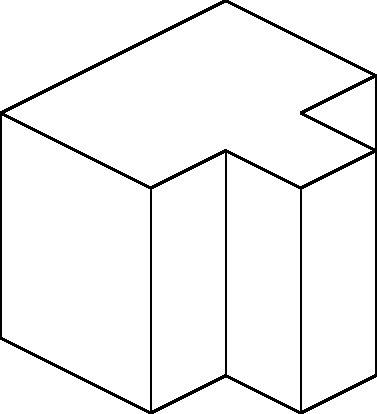
\includegraphics{PSETDISP.pdf}
            \caption{Polygon Set Display}
            \label{psetdisp}
        \end{figure}
 
	\end{enumerate}


	\subsection{Polygon-Set Display Algorithm}
	\label{psetalgo}

	\begin{enumerate}
	\item
	The list of blocks in the component is traversed. The polygons
	contributed by each block are collected.

	\item
	The polygons are grouped together after sorting by the value of the normal
	to the polygon plane.
	
	\item

	These groups of the polygons are further sorted in such a way that all 
	co-planar polygons go to a single polygon set.

	\item
	The first polygon-set in the list of polygon-sets is set as the current
	polygon-set.

	\item
	\label{ploop}
	If the current polygon-set is empty; go to step ~\ref{eimerg}.
	Else, the head of the list of polygons in the current polygon-set is set
	as the current polygon. 

	\item
	The polygon next to the current polygon in the current polygon-set is set
	as the second polygon. 
	\item
	\label{st5}
	Algo.~\ref{mergalgo} is called with arguments as the current polygon and
	the second polygon.

	\item
	If the value returned from Algo. ~\ref{mergalgo} is NULL,
		\begin{itemize}
		\item
			the second polygon is set as the current polygon,
		\item
			the polygon next to the second polygon is set as the second polygon.
		\end{itemize}
	Else, 
		\begin{itemize}
		\item
			the second polygon is removed from the current polygon-set,
		\item
			the polygon next to the second polygon is set as the current 					polygon.
		\end{itemize}
	Step ~\ref{st5} is repeated till the last polygon in the current polygon-set
	becomes the current polygon.

	\item
	\label{eimerg}
	If the polygon-set next to the current polygon-set is NULL,
	\begin{itemize}
	\item
	Go to step ~\ref{pdisp}.
	\end{itemize}
	Else, 
	\begin{itemize}
	\item
	The polygon-set next to the current polygon-set is set as the current
	polygon-set
	\item
	Go to step ~\ref{ploop}.
	\end{itemize}

	\item
	\label{pdisp} 
	All the polygon-sets are traversed and all the polygons in each
	polygon-set are displayed.

	\end{enumerate}

	\subsection{Common Edge Detection Algorithm}
	\label{commalgo}
	\begin{itemize}
	\item
	Input : 
			\begin{itemize}
			\item
			An Edge $E1 (V_{1},V_{2})$ of the {\em first polygon}. 
			\item
			The second polygon.
			\end{itemize}

	\item
	Output: 
			\begin{itemize}
			\item
			If there is a common edge, the vertex P of the second polygon to 
			be traversed next from $V_{1}$ is returned.
			\item
			If there is no common edge, a value of NULL is returned.
			\end{itemize}
	\end{itemize}

	\begin{enumerate}
	\item
	\label{commthree}
	The first edge of the second polygon is made the {\em current edge} and
	is denoted by $E2 (P_{1},P_{2})$.
	\item
	Call $B1 = In-line(P_{1},V_{1},V_{2})$, where $B1$ is a boolean variable.
	$B1$ has value ``true'' if $P_{1}$ lies between $V_{1}$ and $V_{2}$.
	\item
	Call $B2 = In-line(P_{2},V_{1},V_{2})$, where $B2$ is a boolean variable.
	$B2$ has value ``true'' if $P_{2}$ lies between $V_{1}$ and $V_{2}$.
	\item
	Call $B3 = In-line(V_{1},P_{1},P_{2})$, where $B3$ is a boolean variable.
	$B3$ has value ``true'' if $V_{1}$ lies between $P_{1}$ and $P_{2}$.
	\item
	Call $B4 = In-line(V_{2},P_{1},P_{2})$, where $B4$ is a boolean variable.
	$B4$ has value ``true'' if $V_{2}$ lies between $P_{1}$ and $P_{2}$.
        \begin{figure}[htbp]
	% \centerline{\psfig{figure=commedg.ps,width=3.0in,height=4.0in}}
	\hspace{2cm}
	\includegraphics[scale=0.8]{commedg.png}
            \caption{The possible ways of common edge}
            \label{commedg}
        \end{figure}

	\item
	If both $B1$ and $B2$ are ``true'' then the point ($P_{1}$ or $P_{2}$)
	which is closer to $V_{1}$ is stored in list {\em Plist}(Fig.
	~\ref{commedg}(1)). 
	\item
	If either of $B1$ and $B2$ is ``true'' 
	then the point which can be reached from $V_{1}$ without going over the
	common edge is added to {\em Plist}(Fig.~\ref{commedg}(2) and 
	~\ref{commedg}(3)).

	\item
	\label{commfive}
	If both $B3$ and $B4$ are ``true'' then the point
	which is closest to $V_{1}$ than $V_{2}$ is added to {\em Plist}
	(Fig.~\ref{commedg}(4)).
	\item
	\label{commei}
	The next edge of the second in the direction of traversal is made the 
	{\em current edge}.
	If the {\em current edge} is not the first edge in the {\em second polygon},
	steps ~\ref{commthree} to ~\ref{commei} are repeated.

	\item
	The point P in {\em Plist} which is closest to $V_{1}$ and can be reached
	without going over a common segment between the two polygons is returned. 
	If {\em Plist} is empty, return NULL.

	\end{enumerate}

	\subsection{Algorithm for function In-line(edge $E1 (V_{1},V_{2})$,
	vertex $P_{1}$)}
	\label{inline}
	\begin{itemize}
	\item 
	Output: 
			\begin{itemize}
			\item 
			``true'' if $P_{1}$ lies between $V_{1}$ and $V_{2}$
			\item
			``false'' if $P_{1}$ does not lie between $V_{1}$ and $V_{2}$.
			\end{itemize}
	\end{itemize}

    \begin{enumerate}
        \item
        Compute distance $D1$ between $P_{1}$ and $V_{1}$
        \item
        Compute distance $D2$ between $P_{1}$ and $V_{2}$
        \item
        Compute distance $D3$ between $V_{1}$ and $V_{2}$
        \item
        If $ D3 = D1 + D2 $, 
			\begin{itemize}
			\item return ``true''. 
			\end{itemize}
		Else,
			\begin{itemize}
			\item return ``false''. 
			\end{itemize}
    \end{enumerate}


	\subsection{Merging of the polygons}
	\label{mergalgo}

		\begin{itemize}
		\item
		Input : Polygons $P_{1}$, $P_{2}$.
		\item
		Output:	A merged polygon $P_{1}$, or NULL.
		\end{itemize}

		\begin{enumerate}

		\item
		\label{mone}
		Select the first vertex $V_{1}$ in $P_{1}$ as the current vertex.
		Set $P_{1}$ as the current polygon, $P_{2}$ as the second polygon.
		Define a new polygon $P$ with $V_{1}$ as its first vertex. Set
		the traversal direction to Forward \footnote{``Forward'' implies
		that the doubly linked list of vertices will be traversed following
		the ``next'' pointer; ``Backward'' implies that this list will be 
		traversed following the ``previous'' pointers. }.
		Set $NPOLY = 1 $.

		\item
		\label{mtwo}
		Select the edge of the current polygon 
		emanating from the current vertex in the traversal direction as the 
		current edge. Call Algo. ~\ref{commalgo} with arguments as the
		current edge and the second polygon and return value as $V$.
		
		\item
		\label{mthree}
		If $V$ is NULL,
			\begin{itemize}
			\item
			Set the vertex at the other end of the current edge to be the 
			current vertex. 
			\item
			Add the current vertex to $P$. 
			\item
			Go to step ~\ref{mfive}. 
			\end{itemize}
		Else,
			\begin{itemize}
			\item
			Add $V$ to $P$. 
			\item
			Make the second polygon the current polygon. 
			\item
			Make the current polygon the second polygon. 
			\item
			Make $V$ the current vertex.
			\item
			Set the traversal direction to be such that the next edge traversed
			from $V$ will not contain the common segment $S$. 
			\item
			Go to step ~\ref{mfive}.
			\end{itemize}

		\item
		\label{mfive}
		If the current vertex is the starting vertex $V_{1}$, 
			\begin{itemize}
			\item
			Go to step ~\ref{msix}.
			\end{itemize}
		Else, 
			\begin{itemize}
			\item
			Go to step ~\ref{mtwo}.
			\end{itemize}
		\item
		\label{msix}
		If $NPOLY = 1$, 
			\begin{itemize}
			\item
			$P1 = P$.
			\item
			Return $P1$.
			\end{itemize}
		Else,
			\begin{itemize}
			\item
 			Add $P$ to the bottom of the polygon-set.
			\item
			$NPOLY = NPOLY + 1$.
			\end{itemize}
		\item
		\label{mseven}
		If $P_{1}$ contains any vertices not in $P$,
			\begin{itemize}
			\item
			Set $V_{1}$ to be such a vertex.
			\item
			Go to step ~\ref{mtwo}
			\end{itemize}
		Else, if $P_{2}$ contains any vertices not in $P$,
			\begin{itemize}
			\item
			Set any such vertex as the current vertex.
			\item
			Go to step ~\ref{mtwo}
			\end{itemize}
		Else,
			\begin{itemize}
			\item
			Exit.
			\end{itemize}
		\end{enumerate}

